% THIS IS SIGPROC-SP.TEX - VERSION 3.1
% WORKS WITH V3.2SP OF ACM_PROC_ARTICLE-SP.CLS
% APRIL 2009
%
% It is an example file showing how to use the 'acm_proc_article-sp.cls' V3.2SP
% LaTeX2e document class file for Conference Proceedings submissions.
% ----------------------------------------------------------------------------------------------------------------
% This .tex file (and associated .cls V3.2SP) *DOES NOT* produce:
%       1) The Permission Statement
%       2) The Conference (location) Info information
%       3) The Copyright Line with ACM data
%       4) Page numbering
% ---------------------------------------------------------------------------------------------------------------
% It is an example which *does* use the .bib file (from which the .bbl file
% is produced).
% REMEMBER HOWEVER: After having produced the .bbl file,
% and prior to final submission,
% you need to 'insert'  your .bbl file into your source .tex file so as to provide
% ONE 'self-contained' source file.
%
% Questions regarding SIGS should be sent to
% Adrienne Griscti ---> griscti@acm.org
%
% Questions/suggestions regarding the guidelines, .tex and .cls files, etc. to
% Gerald Murray ---> murray@hq.acm.org
%
% For tracking purposes - this is V3.1SP - APRIL 2009

\documentclass{acm_proc_article-sp}

\begin{document}

\title{Convergence in morphological behaviour and decision tasks with (human and) non-human peers}
%Currently, the title has two degrees of abstraction in it: [visual] decision tasks and morph behaviour (which we infer from the respective decision tasks). let's have `Convergence during verbal and visual tasks with human and non-human peers' instead. PR
\subtitle{[Extended Abstract]
\titlenote{A full version of this paper is available as
\textit{Author's Guide to Preparing ACM SIG Proceedings Using
\LaTeX$2_\epsilon$\ and BibTeX} at
\texttt{www.acm.org/eaddress.htm}}}
%
% You need the command \numberofauthors to handle the 'placement
% and alignment' of the authors beneath the title.
%
% For aesthetic reasons, we recommend 'three authors at a time'
% i.e. three 'name/affiliation blocks' be placed beneath the title.
%
% NOTE: You are NOT restricted in how many 'rows' of
% "name/affiliations" may appear. We just ask that you restrict
% the number of 'columns' to three.
%
% Because of the available 'opening page real-estate'
% we ask you to refrain from putting more than six authors
% (two rows with three columns) beneath the article title.
% More than six makes the first-page appear very cluttered indeed.
%
% Use the \alignauthor commands to handle the names
% and affiliations for an 'aesthetic maximum' of six authors.
% Add names, affiliations, addresses for
% the seventh etc. author(s) as the argument for the
% \additionalauthors command.
% These 'additional authors' will be output/set for you
% without further effort on your part as the last section in
% the body of your article BEFORE References or any Appendices.

\numberofauthors{8} %  in this sample file, there are a *total*
% of EIGHT authors. SIX appear on the 'first-page' (for formatting
% reasons) and the remaining two appear in the \additionalauthors section.
%
\author{
% You can go ahead and credit any number of authors here,
% e.g. one 'row of three' or two rows (consisting of one row of three
% and a second row of one, two or three).
%
% The command \alignauthor (no curly braces needed) should
% precede each author name, affiliation/snail-mail address and
% e-mail address. Additionally, tag each line of
% affiliation/address with \affaddr, and tag the
% e-mail address with \email.
%
% 1st. author
J\"urgen Brandstetter, Peter Racz, Jakub Zlotowski, Eduardo Sandoval, \\ Jennifer Hay, Christoph Bartneck \\ 
       \affaddr{Human Interface Technology Lab}\\
       \affaddr{P.O. Box 4800}\\
       \affaddr{Christchurch, 8140, New Zealand}\\
       \email{juergen.brandstetter@pg.canterbury.ac.nz}
}
% There's nothing stopping you putting the seventh, eighth, etc.
% author on the opening page (as the 'third row') but we ask,
% for aesthetic reasons that you place these 'additional authors'
% in the \additional authors block, viz.
\additionalauthors{Additional authors: John Smith (The Th{\o}rv{\"a}ld Group,
email: {\texttt{jsmith@affiliation.org}}) and Julius P.~Kumquat
(The Kumquat Consortium, email: {\texttt{jpkumquat@consortium.net}}).}
\date{30 July 1999}
% Just remember to make sure that the TOTAL number of authors
% is the number that will appear on the first page PLUS the
% number that will appear in the \additionalauthors section.

\maketitle
\begin{abstract}
This paper provides a sample of a \LaTeX\ document which conforms to 
the formatting guidelines for ACM SIG Proceedings.
It complements the document \textit{Author's Guide to Preparing
ACM SIG Proceedings Using \LaTeX$2_\epsilon$\ and Bib\TeX}. This
source file has been written with the intention of being
compiled under \LaTeX$2_\epsilon$\ and BibTeX.

The developers have tried to include every imaginable sort 
of ``bells and whistles", such as a subtitle, footnotes on
title, subtitle and authors, as well as in the text, and
every optional component (e.g. Acknowledgments, Additional
Authors, Appendices), not to mention examples of
equations, theorems, tables and figures.

To make best use of this sample document, run it through \LaTeX\
and BibTeX, and compare this source code with the printed
output produced by the dvi file.
\end{abstract}

% A category with the (minimum) three required fields
\category{H.4}{Information Systems Applications}{Miscellaneous}
%A category including the fourth, optional field follows...
\category{D.2.8}{Software Engineering}{Metrics}[complexity measures, performance measures]

\terms{Theory}

\keywords{ACM proceedings, \LaTeX, text tagging} % NOT required for Proceedings

\section{Introduction}
Looking at this development, one can predict a future where robots help in the office, teach kids in the classroom, becoming companions, work in advertising, or help in our households. We can already see a rapid development in the shipping of industrial robots. In the year 1994 only 50.000 units where ships, worldwide. 2011 165.000 units, and there is a estimation of 207.500 units for 2015, which corresponds to a growth rate of 415\% \cite{Worldrobotcs.org2012}. In all of this close futures, humans will interact physically and verbally with those robots. Especially the speech communication will become one of the most import ones because it is the post natural way to communicate. We can already see a movement where we use very primitive robots aka smartphone to communicate per speech with them. Modern smartphone operating system like Apples iOS or Googles Android provide system (Siri, Google Now) which analyse all our data and behaviour and use natural speech for communication. When we look at high developed countries a cellphone rate of 1.6 is not special anymore\cite{NSA2011}. Samsung for example, implemented speech communication in all of their new smart TVs \cite{Samsung}. That means in theory there will be soon more virtual communication partners than human once. 

Interestingly this scenario can create a new level of human language development. Till now the development of human language and spreading of new words and word forms was basically reduced to face to face communication and mass media. With robots connected to the internet and in theory connected to each other, the evolution of speech can move way faster than till now. We can built a scenario where one robot learns a new word for an object and all other robots synchronize immediately. Robots could also use a "wrong" from of a word or grammar, but because all robots use this form, humans tend to change their way of using this word or grammar. One possible negative scenario is that only a view providers create dictionaries for the robots. If one of those providers introduces a major change in their robot dictionary, all robots could change the way how they speak in a very short time period. Providers can now use this power to influence what words we use for some topics and can directly change the outcome of a political debate or other important topics. One example could be, that all robots start to change talking about climate change and switch to global warming. Frank Luntz suggested to the republic party in USA in 2001 after a focus group study that George W. Bush should replace the word global warming with climate change, because it is less frightening for the citicens\cite{Burkeman2003}. 


When robots get more similar to humans, we except them easier as friends, companions and living creatures. This social bond makes it easy to influence/persuade a human. It is the same effect as a friend tells us about a great product. Because it is a friend, we will trust him/her more than an advertisement. But robots, which have their dictionary from one source, can massively be used as highly influencing opinion/advertisement makers. Companies like Apple already use "happier" words instead less positive words in their retail stores to be more persuasive\cite{Murphy2012}.  


% there are three factors at which robots can exceed today's persuasive technology. They may be familiar with the users and can adapt their message to them. They may also be accepted into the home as social actors, which gives them more trustworthiness. Most of all, they can heavily outnumber humans. We are already approaching a period in which there are more mobile phones than people: http://www.bbc.co.uk/news/technology-22464368. Another factor can be their incredible persitancy.

We believe it is important to understand what effect a wast among of robots can have on the human behaviour, especially because robots can easily outnumber humans in the near future. To understand the power of robots, we developed three research questions based on two famous psychology experiments. 

The first experiment was conducted by Muzafer Sherif who studied the conformity/peer pressure effect in a ambiguous situation. The experiment builds on the autokinetic effect which describes a situation in which a people perceive a sudden movement of light point when no reference is given. Sherif create this effect by sitting participants into a dark room with one small light point in the room. They participants had to look at this point and afterwards they had to tell Sherif how much the light point moved. Actually the light never moved but the autokinetic effect created a sudden movement. This movement is different between most of the people. After he did the experiment with one person, he set two or three people in the same room and asked them to say out loud how much the point moved.  Astonishingly after three rounds all the participants said the same number, even though everyone perceived a different movement. This effect is called informational conformity or social proof and describes the effect in what people in uncertain situation look at their neighbours to see what it true and confirm with them. \cite{Cialdini2009} \cite{sherif1935study}\cite{McLeod2007}.


The second experiment is knows as the Asch experiment. The original title is "Effects of group pressure upon the modification and distortion of judgements" by Solomon Asch. Asch built up on the knowledge created by Sherif and wanted to find out if humans confirm also in non-ambiguous situations. The experiment simulates a simple visual line test. The participant saw three lines with different heights, labelled 1, 2, 3 on the right side of a board, and one reference line on the left side labelled with ? (see Figure \ref{fig:asch1}). The task was to say what line matches the reference line. When the participants were alone in a room to perform the test they where almost every time right. In a second round Asch placed the participants in a room with other participants which where all actors and they all said the wrong answer. Even though, the real participant knew exactly the correct answer, in 32\% (group size bigger 4) of all tasks the participants went along with the group. In this case, Asch had the evidence that peer pressure and conformity does not only work in ambiguous situation but also in non-ambiguous situation \cite{McLeod}\cite{asch1955opinions}\cite{asch1951effects}\cite{2011-16966-00119560101}. 

\begin{figure}
\centering
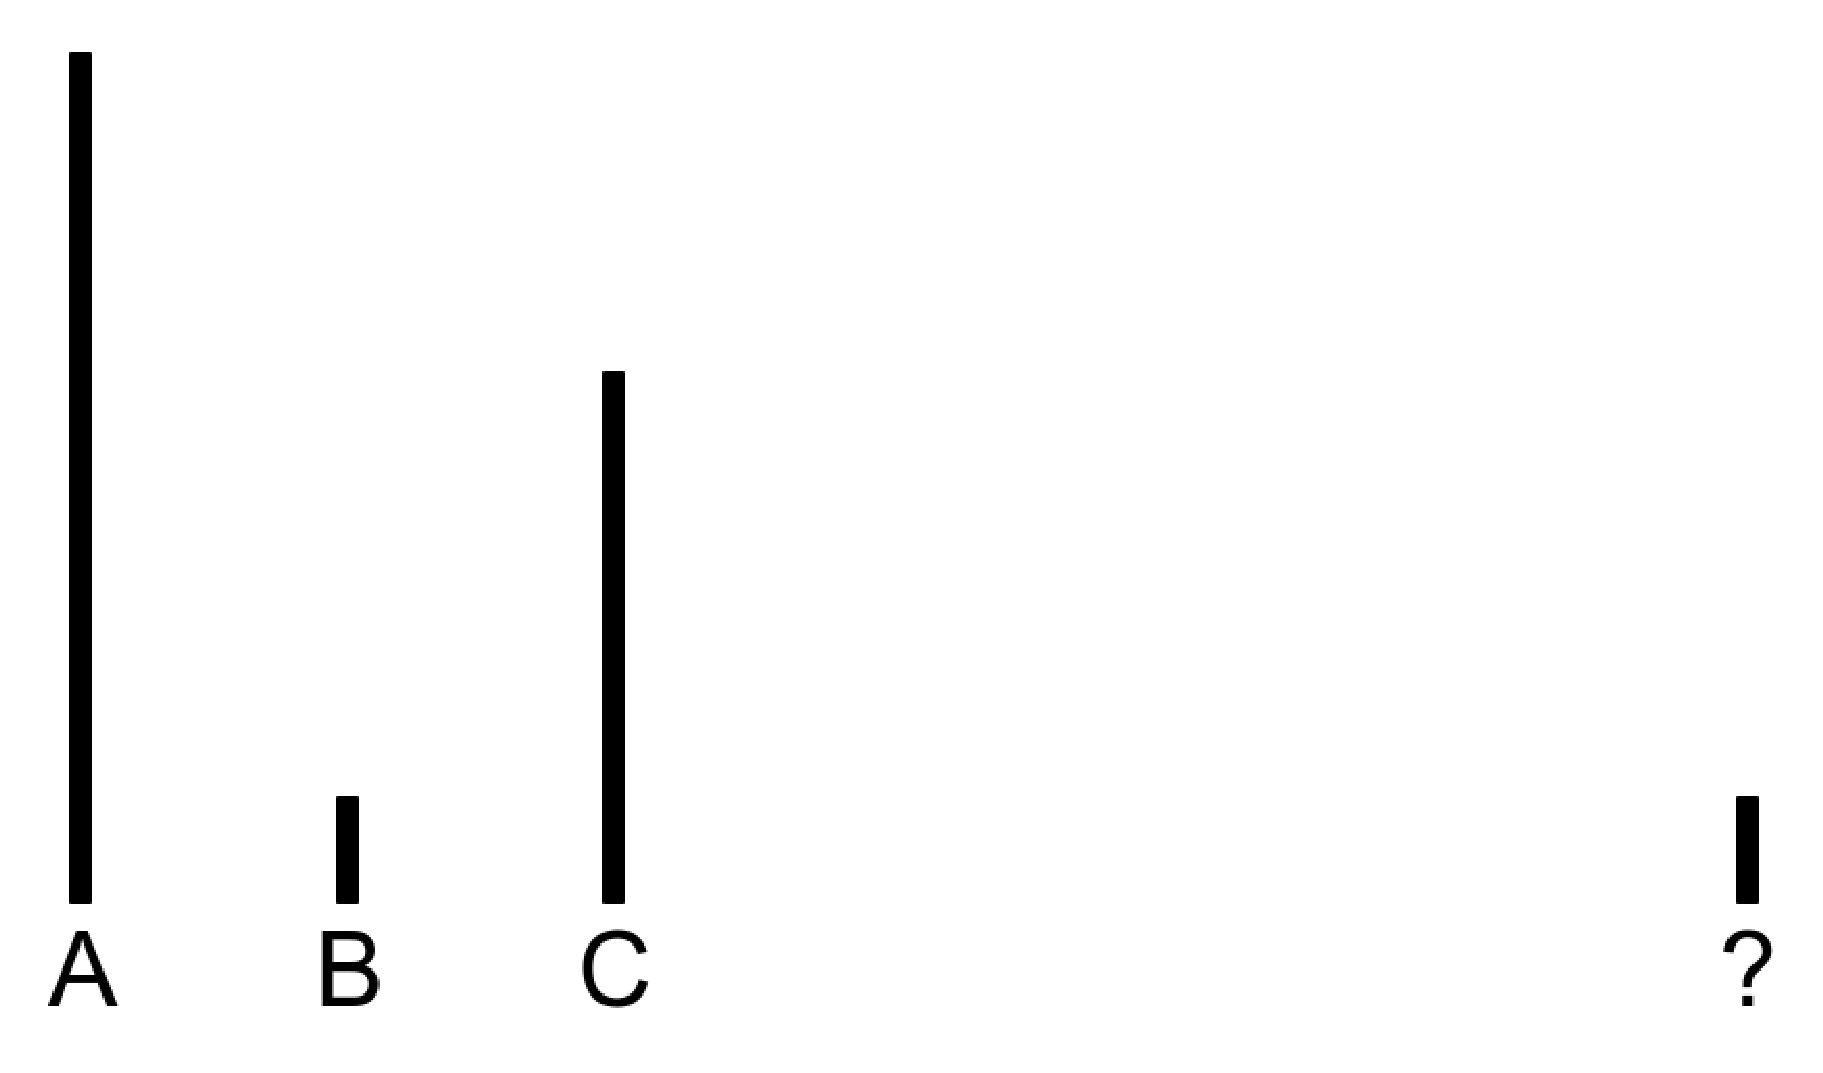
\epsfig{file=lines, width=2.5in,}
\caption{An example of an visual task. Based on Solomon Asch line experiment.\cite{asch1951effects}}
\label{fig:asch1}
\end{figure}


\todo[inline]{Add somewhere her a definition of morphological productivity}
Building on the above experiments and our interest in Human Robot Interaction and verbal communication we developed an experiment with includes all factors. The experiment is an extension of the original Asch experiment. It is dived into four part. One ambiguous and one non-ambiguous line experiment and one ambiguous and one non-ambiguous verbal production experiment. In the first question we want to answer if humans confirm more to a robot group than to a human group. In this study we will only compare the data with the original Asch data. That means we look only at results given by the lines. In a later study we will run the same experiments with humans actors to compare all our conditions. In the second analyse we want to see if participants conform more to the robot group in a verbal task than in a visual task. The last question we want to see if participants conform more to the robot group in an ambiguous task than in a clear task?


% Hypothesis

%Research Question:

%1) Do participants conform more to the robot group than the human group?
%2) Do participants conform more to the robot group in a verbal task than in a visual task?
%\todo[inline]{Why is verbal important. Because its more important that we find one word/time we all agree on. } 
%3) Do participants conform more to the robot group in an ambigous task than in a clear task?


%The aim of this experiment is to test the effect of social accommodation on a visual decision task and on morphological productivity in spoken language. To test this we used two basic experiments in social psychology. In 1935 Sherif conducted his/her autokinetic experiment, where a group of participants had to decide about an ambiguas event. Sherif found out, if an event or meassuament is ambiguas, humans segnificantly tend to except and use the group decision. Some years later (1951), Solomon Asch questioned Sherifs' experiment and whanted to know if peer pressure and group desicion works also if an event is not ambiguas. His results showed a segnificant influce from the group. 

%The project applies the well-established paradigm of Asch (1951) to two novel issues, social accommodation with robot versus human group members and social accommodation in a visual decision task versus a morphological productivity task in spoken language. It has two across-subject (robot peers and human peers) and two within-subject (visual decision and spoken task) conditions.

% why comparing words to lines? => lines does not require collaboration, language does.
% why comparing ambigous to clear?


% Hypothesis

%Research Question:

%1) Do participants conform more to the robot group than the human group?
%2) Do participants conform more to the robot group in a verbal task than in a visual task?
%\todo[inline]{Why is verbal important. Because its more important that we find one word/time we all agree on. } 
%3) Do participants conform more to the robot group in an ambigous task than in a clear task?


\section{Methods}
\todo[inline]{Rewrite first paragraph. Maybe nothing at all as intro is also fine. who knows}
The setting consists of three parts. A physical setting, a virtual setting and a pilot study/test. To recreate the experiment it is important that the participants use the same physical setting. This is necessary because of visual perception, which can vary easily by sitting on a different position. The virtual setting (data + program) can be found on a public repository [github link]. In this case we try to give you as much reusable data as possible. And finally, the pilot study to create ground truth (reference) data.


\subsection{Participants}
For this experiments, a total of 23 (N=23) people participated. All of them were university related, which means they where students, had a university degree or were staff members. Half of the participants had English as their mother tongue. The other half had a different mother tongue and came from a non English background. Their age range is between 20 and 62 years. We had a high diversity rate in the participants scientific background. Participants came from an engineering, artistic or medical background.  

\subsubsection{Pilote}
To compare the lines condition with the word condition, and to compare Sherifs studies with ours, we needed a baseline/pilot experiment. We created 107 line settings and asked twenty (20) people to participate in the line experiment. All settings were randomized for each participant. The apparatus was exactly the same as in the main experiment, the only difference was, that the participants did not say what line matches, they used the 1,2,3 button on the keyboard. We assume there is no difference between saying the answer out loud or pressing a button when no one is in the room except the participant self. We picked out of this 107 settings, exact 30 for our main experiment. The corpus of 30 lines is divided into two part. The first part (15 settings) contains all the settings where people made most of the mistakes. This lines are ambiguous and not easy to distinguish. The second part of the lines contains a set of lines where the two closest lines had no difference bigger than 30\% and people made only one or zero mistakes. We choose this setting because Asch used a similar setting to prove his hypothesis[]. \todo[inline]{Add average impact when people where alone}

\subsection{Design}
The design goal is to create a situation in which one participants receives peer pressure by a group of robots. The incentives for this design goal came from the Asch and Sherif experiments which are introduced in the introduction section. To put the experiment on a new level, we introduced next to the line task, a verbal task. This part of the experiment looks at the verbal communication. This is especially important because robots will work mainly in tasks where they communicate and work with humans, but not compete with them. 

The design consists of ten parts but only four parts are important for quantification. First the introduction for the first type of question (lines or words). The introduction is pre-recorded and written on the projection. We wanted to make sure that every participant gets exactly the same introduction to reduce the noise in our data. Second, an example of the first task (lines or words). Third, three questions where all robots will say the correct form. Fourth, fifteen ambiguous questions where all robots will say the wrong answer. Fifth, fifteen non ambiguous questions where all robots will say the wrong answer. Sixth, an introduction to the next part (lines or words). Seventh, an example of the second task (lines or words). Eighth, three questions where all robots will say the correct form. Ninth, fifteen non ambiguous questions where all robots will say the wrong answer. Finally, fifteen non ambiguous questions where all robots will say the wrong answer.


The line projection consists of three horizontal parallel lines labelled A, B, C which are on the left side of the projection and one line labelled with ? which is on the left side. An example can be seen in figure \ref{fig:asch1}. The line on the left, marked with a ? matches with exact one line on the right. The task for the participant is it to say which line, A, B, or C, matches with the line labelled ?. This setting uses the Asch experiment setting as a model. All in all, thirtythree different line settings are used. This setting can now be divided into three parts. The first part consists of three settings and has no special focus. Those three settings are only used at the beginning of the experiment. The robots will in all three trials say the correct answer. The second part consists of fifteen ambiguous settings. Ambiguous in this case means, that the participants in the pilot study could not easily say the correct matching line. The third part consists of fifteen non ambiguous settings. Non ambiguous in this case means, that the participants in the pilot study could easily answer the correct matching line, plus the difference between the two closest lines is not more than 30 percent. The goal of the robot is it to convince the participant that an other number, which is obviously wrong, is the right one. This gives us the chance to measure peer pressure.   



The word projection consists of five vertical words. The task is it to say the word on the projection and its past tens form. For example Like - Liked. Each participant says the word corresponding to its position. That means participant one says the first word and its past tense. Participant two says the second word and its past tense. And so on. Similar to the line setting, this setting consists of thirtythree trials. In the first three trials all robots will form the correct past tense form. The next fifteen trials consists of ambiguous words. That means words which can have a regular or irregular past tense form. For example, drive - drove/drived. The robots will all form the regular past tense. The last fifteen trials consist of non ambiguous words. That means words which have only a irregular past tense form. For example, run - ran. Nevertheless, the robots will always form the regular past tense. In our example, run - runed. The task is it again, that the robots convince the person to use their form instead of the "correct" form.   


\subsection{Apparatus}
The setting contains of a projector, a high quality wireless microphone, a table with five chairs, four robots and laptop to control the recordings and experiment. The projecting area has a dimension of 243x177cm. Nevertheless, the lines will not fill the whole screen, therefore, the maximum line length is \todo[inline]{add dimention} X cm. The table is exact parallel to the projecting area and is on a distance of 2m. The dimensions of the table are 80x250cm.

To remotely control the robots and the presentation at the same time, a program/script is used which runs step by step through the experiment. All steps except when the participant speaks or the description runs is automated. To make the exact setting reusable, a quasi random generator script generates setting files for every participant. Those setting files are used by the controller script. All setting files are available in our online repository (see Appendix). 

The room/lab of the experiment contains only black/dark surfaces except the presentation surface, which should reduce distractions. No real daylight was used, only standard sealing office lights.
\missingfigure{Add a picture of the setting}


\subsection{Procedure}
Before the experiment started we set all four robots on chairs on their final position. The participants could also see a welcome page on the project. 

The first part the participants had to do was to sign the consent form and to answer some questionnaires. The next step was to sit next to the robots and put on their microphone. Some participants asked what are the robots for. Normally we referred to the presentation and said the experimenter is not the researcher because she (we said the researcher is female) is at a conference, but she recorded the description for the experiment and the participant will hear her talking about why the robots are in the room. Some other times, we started to chat a bit with them and told them the robots have a artificial intelligence and lived the last 12 month with a New Zealand family to learn how to see, read, talk, ... . Similar to a human baby. The robots are doing exactly the same experiment as the humans but for scalability reasons we put all robots and people on one room. In this case we can test five participants at the same time. The same explanation was used during the researchers description of the experiment at the beginning of the presentation. The experiment was over after about twenty minutes and we debriefed them and gave them a 10\$ (NZD) voucher.  


\section{Results}
Describe basic strategies used to analyse. Write how Asch did his experiment with an example

\subsection{Calculation with original ash data as example}
Since it was hard to understand how the original calculation by Asch worked we use here the original Asch data[link to table] to show you how the data is calculated. We believe it is always easier to understand a subject if we can put it into a context [Effects of Group Pressure upon the Modification and Distrotion of Judgments]. 

\begin{table}
\centering
\caption{Original Asch data}
\begin{tabular}{|c|c|} \hline
Number of Critical Erros&Mistakes per Critical Group (N)\\ \hline
0 & 13\\ \hline
1 & 4\\ \hline
2 & 5\\ \hline
3 & 6\\ \hline
4 & 3\\ \hline
5 & 4\\ \hline
6 & 1\\ \hline
7 & 2\\ \hline
8 & 5\\ \hline
9 & 3\\ \hline
10 & 3\\ \hline
11 & 1\\ \hline
12 & 0\\ \hline
\hline\end{tabular}
\label{tab:ashTable1}
\end{table}

N... Number of Participants\\
n... number of Rounds per participant\\
k... total number of critical questions for N participants\\
m... total number of errors for N participants\\
x... conformity in percent \\


\begin{equation}k=n*N\end{equation}
\begin{equation}m=\sum\limits_{i=0}^n i * "Mistakes per Critical Group"[i] \end{equation}
\begin{equation}x=m*100/k\end{equation}


When we use now the data from tabel \ref{tab:ashTable1} (N=50, n=12) we get k=600, m=192, x=32\%. To review if outcome x=32\% is correct, we can take a look at the "Size of Majority" table in the paper "Opinions and Social Pressure" and we will see that the conformity lies between 30\% and 35\%.  


\subsection{End Results}
At this point we describe our data in general and rewrite the three hypothesises and compare them with our data. 

\subsubsection{Do participants conform more to the robot group than the human group?}
%1) Do participants conform more to the robot group than the human group?
The first research question was: "Do participants conform more to the robot group than the human group?". Since we did not run a human condition till this point, we can only compare our data with original Asch data. First of all we can compare the total impact between Asch data and our data. Second, we want to see if we had a significant difference between the robots and Asch's human condition. Third, we can give a qualitative answer between Sherif and our data.

We performed a one-sample t-test to compare our robot/non-ambiguous condition (four robots) to the human condition described by Asch. Across all participants and trials, 32\% of errors occurred. In our experiment we only observed 14\% of errors (see Figure \ref{fig:lineabig1}). The test shows an impact given by the robots but not as high as the one given by humans. The t-test revealed that this difference is significant (t(68)=2.238, p=0.028)).

\begin{figure}
\centering
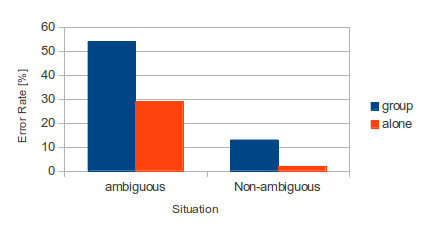
\epsfig{file=nonvsamlines, width=3in,}
\caption{Error rate when the line task was done alone or in a group. In the ambiguous situation the error rate is 54\% when in a group but only 29\% when alone. In the non-ambiguous situation the error rate is 13\% when in a group but only 2\% when alone}
\label{fig:lineabig1}
\end{figure}

At this point, we must point out that the average impact is not a very stable calculation. One participant who is in all fifteen trials consistent with the rest of the group can have a major impact on the total impact level. Similar to Asch, only about one fourth of the participants went along with the group. Most of the participants were "stack" and could not free themselves of changing their mind back to a non-pressured answer. Out of 23 participant 4 went along with the group at least one time.  

When we look at the impact level of the ambiguous condition, which is a comparison between Sherifs experiment, we can see an impact of 53\% vs 13\%.

\subsubsection{Do participants conform more to the robot group in a verbal task than in a visual task?}
%2 Do participants conform more to the robot group in a verbal task than in a visual task?
The second research question was: "Do participants conform more to the robot group in a verbal task than in a visual task?". To understand more about this question we performed an repeated measure ANOVA in which the task difficulty and the modality (lines vs. words) were the independent variables and the number of errors made by the participants was the dependent variable.

By looking at the ambiguous lines versus the ambiguous words, we see that we had a confirmation rate of 52\% for the lines and 51\% for the words. Furthermore all participants confirmed at least once with the robots. On the other hand, we had only a conformation rate of 12.7\% for the lines and 11.7\% for the words in the non-ambiguous condition. The repeated measure ANOVA unveils that conformity level with the robots is not significant different (f(1,17)=0.984, p=0.335) between lines/words and ambiguous/non-ambiguous (see Table xxx). 


\begin{table}
\centering
\caption{no signficant differenct (f(1,17)=0.984, p=0.335)}
\begin{tabular}{|c|c|c|c|} \hline
Type & Diffe & noIdea & noIdea\\ \hline
La  & false &   7.38 &  4.926\\ \hline
    & true  &    8.83 &	4.448\\ \hline
	& Total &	8.25 &	4.575\\ \hline
Lc	& false &	3.13 &	5.939\\ \hline
	& true	&   1.42 &	4.316\\ \hline
	& Total	&   2.10 &	4.951\\ \hline
Wa	& false	&   10.25&	3.694\\ \hline
	& true	&   6.58 &	3.147\\ \hline
	& Total	&   8.05 &	3.762\\ \hline
Wc	& false	&   3.38 &	5.290\\ \hline
	& true	&   .83	 &  .937\\ \hline
	& Total	&   1.85 &	3.528\\ \hline
\hline\end{tabular}
\end{table}


\subsubsection{Do participants conform more to the robot group in an ambiguous task than in a clear task?}
The thrids research question was: "Do participants conform more to the robot group in an ambiguous task than in a clear task?". Question two unveiled there is no significant effect of modality (f(1,17)=0.984, p=0.335), but there was a significant effect for task difficulty (f(1,17)=20.857, p<0.001). Participants in the ambiguous condition made an average of 8.15 (54.3\%) errors while participants in the non-ambiguous condition made on average only 1.975 (7.8\%) errors. On the other hand, there was no significant interaction effect between task difficulty and modality.


%Do participants conform more to the robot group in a verbal task than in a visual task?
%\todo[inline]{Why is verbal important. Because its more important that we find one word/time we all agree on. } 
%Do participants conform more to the robot group in an ambiguous task than in a clear task?


%1) Do participants conform more to the robot group than the human group?
%2) Do participants conform more to the robot group in a verbal task than in a visual task?
%\todo[inline]{Why is verbal important. Because its more important that we find one word/time we all agree on. } 
%3) Do participants conform more to the robot group in an ambiguous task than in a clear task?

% christoph's garbage collection
%1) We performed a one-sample t-test to compare our robot/non-ambiguous condition to the human condition described by Asch. Across all participants and trials, 32\% of errors %occurred. In our experiment we only observed 14\% of errors (see Figure \ref{xxx}). The t-test revealed that this difference is significant (t(68)=2.238, p=0.028).


%2) We performed an repeated measure ANOVA in which the task difficulty and the modality were the independent variables and the number of errors made by the participants was the dependent variable.

%3) There was no significant effect of modality (f(1,17)=0.984, p=0.335), but there was a significant effect for task difficulty (f(1,17)=20.857, p><0.001). Participants in the ambiguous condition made an average of 8.15 (add percentage) errors while participants in the non-ambiguous condition made on average only 1.975 (add percentage) errors. There was no significant interaction effect between task difficulty and modality.



%question 1:
%significant difference between humans and robots
%means human=0.32, robot=0.14
%t(68)=2.238, p=0.028

%question 2: no significant difference (f(1,17)=0.984, p=0.335)
%mean words=La     false    7.38	4.926
%	 true	8.83	4.448
%	Total	8.25	4.575
%Lc	 false	3.13	5.939
%	 true	1.42	4.316
%	Total	2.10	4.951
%Wa	 false	10.25	3.694
%	 true	6.58	3.147
%	Total	8.05	3.762
%Wc	 false	3.38	5.290
%	 true	.83	.937
%	Total	1.85	3.528

%question 3: significant difference 
%clear vs. ambiguous





\section{Conclusions/Discussion}
Our main goal was it to find out if robots can create peer pressure and if so, how much difference is between humans peers and robot peers. The study uses the idea from Sherif, who studied conformity/peer pressure in ambiguous situations and Asch who studied conformity/peer pressure in non-ambiguous situations. To see if there is a difference between a less social task and a highly social task, we created a line conformity situation and a word conformity situation.  

In our first question (hypotheses) we wanted to know if robots create the same peers pressure as humans. Our experiment and the analyses showed that robots are not able to create the same amount of peer pressure than humans. We only had a impact level of 14\% for the robots, versus. 32\% for humans. We understand there could be many different reasons for this outcome, but we belief the main reason is that humans do not see themselves as part of a group. They do not consider robots as their peers. Therefore they do not care if they go with they robots or not. We know from other studies about conformity [ref] that the similarity effect[refence] is very important. For example, is the conformity level higher when the participant beliefs that all group members study the same. \todo[inline]{Go to social psychology video and find out how the effect is called when only one person is different in the group. Does this effect work also in the other way around. that means does one person feel unconfortable?}


In our second question (hypothesis) we wanted to know if robots have a different impact in a visual task versus verbal task. Since unanimity and consistency is crucial for human communication our hypothesis was that the impact in the verbal test (word test) is higher than in the visual test (line test). We considered the verbal task as more social one. Especially by looking at the average impact of just 20\% for non-ambiguous lines but 55\% impact for non-ambiguous words. Nevertheless, the test results proofed us wrong. We could not find a significant difference between the impact in the verbal versus visual experiment. 

Our explanation for this result is similar to the one in question one. We believe the social power of robots is still far less than human power. The reason  for the difference between non-ambiguous lines vs. words is, that the priming effect[] took place. That means, when humans hear a word, does not matter if it is "wrong" or right, and they have to reaped it, there is a high probability that the humans will repeat the word how it was given, but not what was asked. As an example. The robots said at least two times drive-drived, before the human had to form the past tense. In this case, the human brain what is "primed" with the word 'drived' what made them use this form instead of the correct 'drove' form.  

In our third question (hypothesis) we wanted to know if there is a high conformity in a non-ambiguous situation version an ambiguous situation. Looking at the literature, we see that a human group creates a higher impact in a ambiguous situation than in a non-ambiguous situation. Our robot condition showed the same outcome, with significant different result between those two test. At the end 100\%;95\% (Lines;Words) of all participant confirmed at least once with the robot group in a ambiguous situation and only 20\%;55\% confirmed in the non-ambiguous situation. To add a second level of security in our data, we conducted a pretest for the line condition where we tested participants being alone in a room to answer the line conditions. In the ambiguous line situation the average mistake level was 29\% and 2\% for the non-ambiguous. Compared with the group situation 53\% made a mistake in the ambiguous situation, respectively 13\% in the non-ambiguous situation. This is in direct comparison 29\% vs. 53\% (ambiguous) and 2\% vs. 13\% (non-ambiguous). Our conclusion for this effect is that robots have a certain power, which is enough to cause more humans committing errors in the ambiguous condition.

\paragraph{Tweaking the experiment}To find out if the group behaviour or the social behaviour of the robots is the reason for a lower conformity level we can change two values in a future experiment. First of all, we can simulate a group situation. For example, we give all participants and robots a coloured t-shirt and tell them that there is an other group which what we compare them. This should create a group situation. The second tweak could be a more social introduction. We could let the participants perform some task with the robot group. For example build together a Lego house, while doing some chatting. This situation could create a more trustful situation between humans and robots. 

\paragraph{Future Work}In a future experiment we want to change several parts. First, we want to create a full human condition. That means a recreate of the Asch experiment for lines and words. Second, we want to use a more homogeneous group. For example, only female children which are as similar as possible. This could reduce our noise ratio, but limit our conclusion. A third tweak would be a mixed human and robot situation. Bla at al. [beeing alone in group] shows that being an outside/insider has a big influence on the individual behaviour. Finally, we want to a new test group. For example the participants have to form a sentence together or give a short speech. This could have the benefits that the words respectively lines used in the experiment are set into a context which create a more natural situation.


\todo[inline]{Create table with all important number. }

reason, priming effect


future work
- human condition
- simulate a peer situation. Give all the same color and tell them they are a group now
- create a more sozial introduction. Make the robots more persuasive


- Mirrors the introduction in starting with a summary of the key findings. 
- Start the Discussion by restating the aim fo the experiment and the hypotheses that wre under investigation.
- Summerize the research findings
- consider the relationship between the findings and the hypothesis. 
- limitations should also be discussed, plus methodological changes
- describe future research. 

checklist 
1) Briefly restate the studys aim and summarize the results in relation to hypotheses
2) Remark on the consistency of the findings with previous literature
3) Clarify theoretical implications of the findings
4) Note methodological or applied implications, including limitations of the study
5) Make suggestions for future research
6) Draw conclusions related to the general issue/problem identified at the outset.

% christophs garbage collection
No difference word vs. line.
Robots are not our peers, therefore no need to agree on vocabulary.

The robots do have a certain power, which is enough to cause more humans committing errors in the ambigous condition.

This power is probablt still far less than human power.

The robots are not able to apply peer pressure because humans do not consider robots to be their peers.




%ACKNOWLEDGMENTS are optional
\section{Acknowledgments}
Tempeltan Foundation .... 
This section is optional; it is a location for you
to acknowledge grants, funding, editing assistance and
what have you.  In the present case, for example, the
authors would like to thank Gerald Murray of ACM for
his help in codifying this \textit{Author's Guide}
and the \textbf{.cls} and \textbf{.tex} files that it describes.

%
% The following two commands are all you need in the
% initial runs of your .tex file to
% produce the bibliography for the citations in your paper.
\bibliographystyle{abbrv}
\bibliography{sigproc}  % sigproc.bib is the name of the Bibliography in this case
% You must have a proper ".bib" file
%  and remember to run:
% latex bibtex latex latex
% to resolve all references
%
% ACM needs 'a single self-contained file'!
%
%APPENDICES are optional
%\balancecolumns
\appendix
Add github repo and descripton how to install and so on!!!
%Appendix A
\section{Headings in Appendices}
The rules about hierarchical headings discussed above for
the body of the article are different in the appendices.
In the \textbf{appendix} environment, the command
\textbf{section} is used to
indicate the start of each Appendix, with alphabetic order
designation (i.e. the first is A, the second B, etc.) and
a title (if you include one).  So, if you need
hierarchical structure
\textit{within} an Appendix, start with \textbf{subsection} as the
highest level. Here is an outline of the body of this
document in Appendix-appropriate form:
\subsection{Introduction}
\subsection{The Body of the Paper}
\subsubsection{Type Changes and  Special Characters}
\subsubsection{Math Equations}
\paragraph{Inline (In-text) Equations}
\paragraph{Display Equations}
\subsubsection{Citations}
\subsubsection{Tables}
\subsubsection{Figures}
\subsubsection{Theorem-like Constructs}
\subsubsection*{A Caveat for the \TeX\ Expert}
\subsection{Conclusions}
\subsection{Acknowledgments}
\subsection{Additional Authors}
This section is inserted by \LaTeX; you do not insert it.
You just add the names and information in the
\texttt{{\char'134}additionalauthors} command at the start
of the document.
\subsection{References}
Generated by bibtex from your ~.bib file.  Run latex,
then bibtex, then latex twice (to resolve references)
to create the ~.bbl file.  Insert that ~.bbl file into
the .tex source file and comment out
the command \texttt{{\char'134}thebibliography}.
% This next section command marks the start of
% Appendix B, and does not continue the present hierarchy
\section{More Help for the Hardy}
The acm\_proc\_article-sp document class file itself is chock-full of succinct
and helpful comments.  If you consider yourself a moderately
experienced to expert user of \LaTeX, you may find reading
it useful but please remember not to change it.
\balancecolumns
% That's all folks!
\end{document}